\documentclass[border=2pt]{standalone}
\usepackage{tikz}

\begin{document}
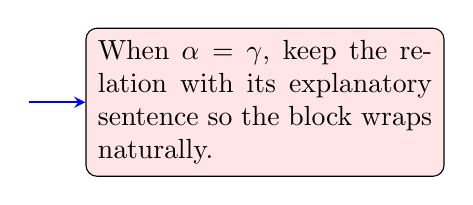
\begin{tikzpicture}
  \node[draw, rounded corners, fill=red!10, inner sep=1ex] (note) at (0,0) {
    \begin{minipage}{0.35\textwidth}
      When $\alpha = \gamma$, keep the relation with its explanatory sentence
      so the block wraps naturally.
    \end{minipage}
  };
  \draw[-stealth, thick, blue] (-3,0) -- (note.west);
\end{tikzpicture}
\end{document}
